\subsection{Observer Pattern}


\subsubsection*{Problembeschreibung}

Häufig müssen verschiedene Komponenten eines Systems synchron gehalten werden. Gleichzeitig soll aber auch eine enge Kopplung dieser Komponenten vermieden werden. Es wird eine $1$:$n$-Beziehung zwischen den Objekten benötigt. Wenn ein Objekt seinen Zustand ändert, so sollen alle abhängigen Objekte benachrichtigt werden, sodass auch sie ihren Zustand aktualisieren können. Ein naiver Lösungsansatz wäre, jedem abhängigen Objekt eine Referenz auf das Objekt zu geben, von welchem es abhängt. Die Objekte könnten dann in regelmäßigen Abständen prüfen, ob eine Zustandsänderung stattgefunden hat. Dieser Ansatz weist jedoch nicht nur eine hohe Kopplung auf, er ist auch wenig performant. Auch wenn keine Zustandsänderung stattgefunden hat, wird auf diese geprüft. Der Aufwand für diese Prüfung steigt dabei linear mit der Anzahl der beteiligten Objekte.

Das Observer-Pattern kann Anwendung finden, wenn es zwei voneinander getrennte Konzepte gibt und eines von dem anderen abhängig ist. Die Abhängigkeit kann modelliert werden, ohne die Objekte zu koppeln. Weiterhin ist es möglich, die Anzahl der abhängigen Objekte variablen zu halten.  

\subsubsection*{Lösung}

Das Observer-Pattern besteht aus einem Publisher und mehreren Subscribern. Die Subscriber implementieren das Subscriber-Interface, welches eine Methode `update`  zur Aktualisierung des Zustandes bereitstellt. Der Publisher hält eine Liste von Referenzen auf Subscriber und verfügt über die Methoden `subscribe` und `unsubscribe`, welche es ermöglichen, der Liste Subscriber hinzuzufügen, oder sie zu entfernen. 

\begin{figure}[!hb]
	\centering
	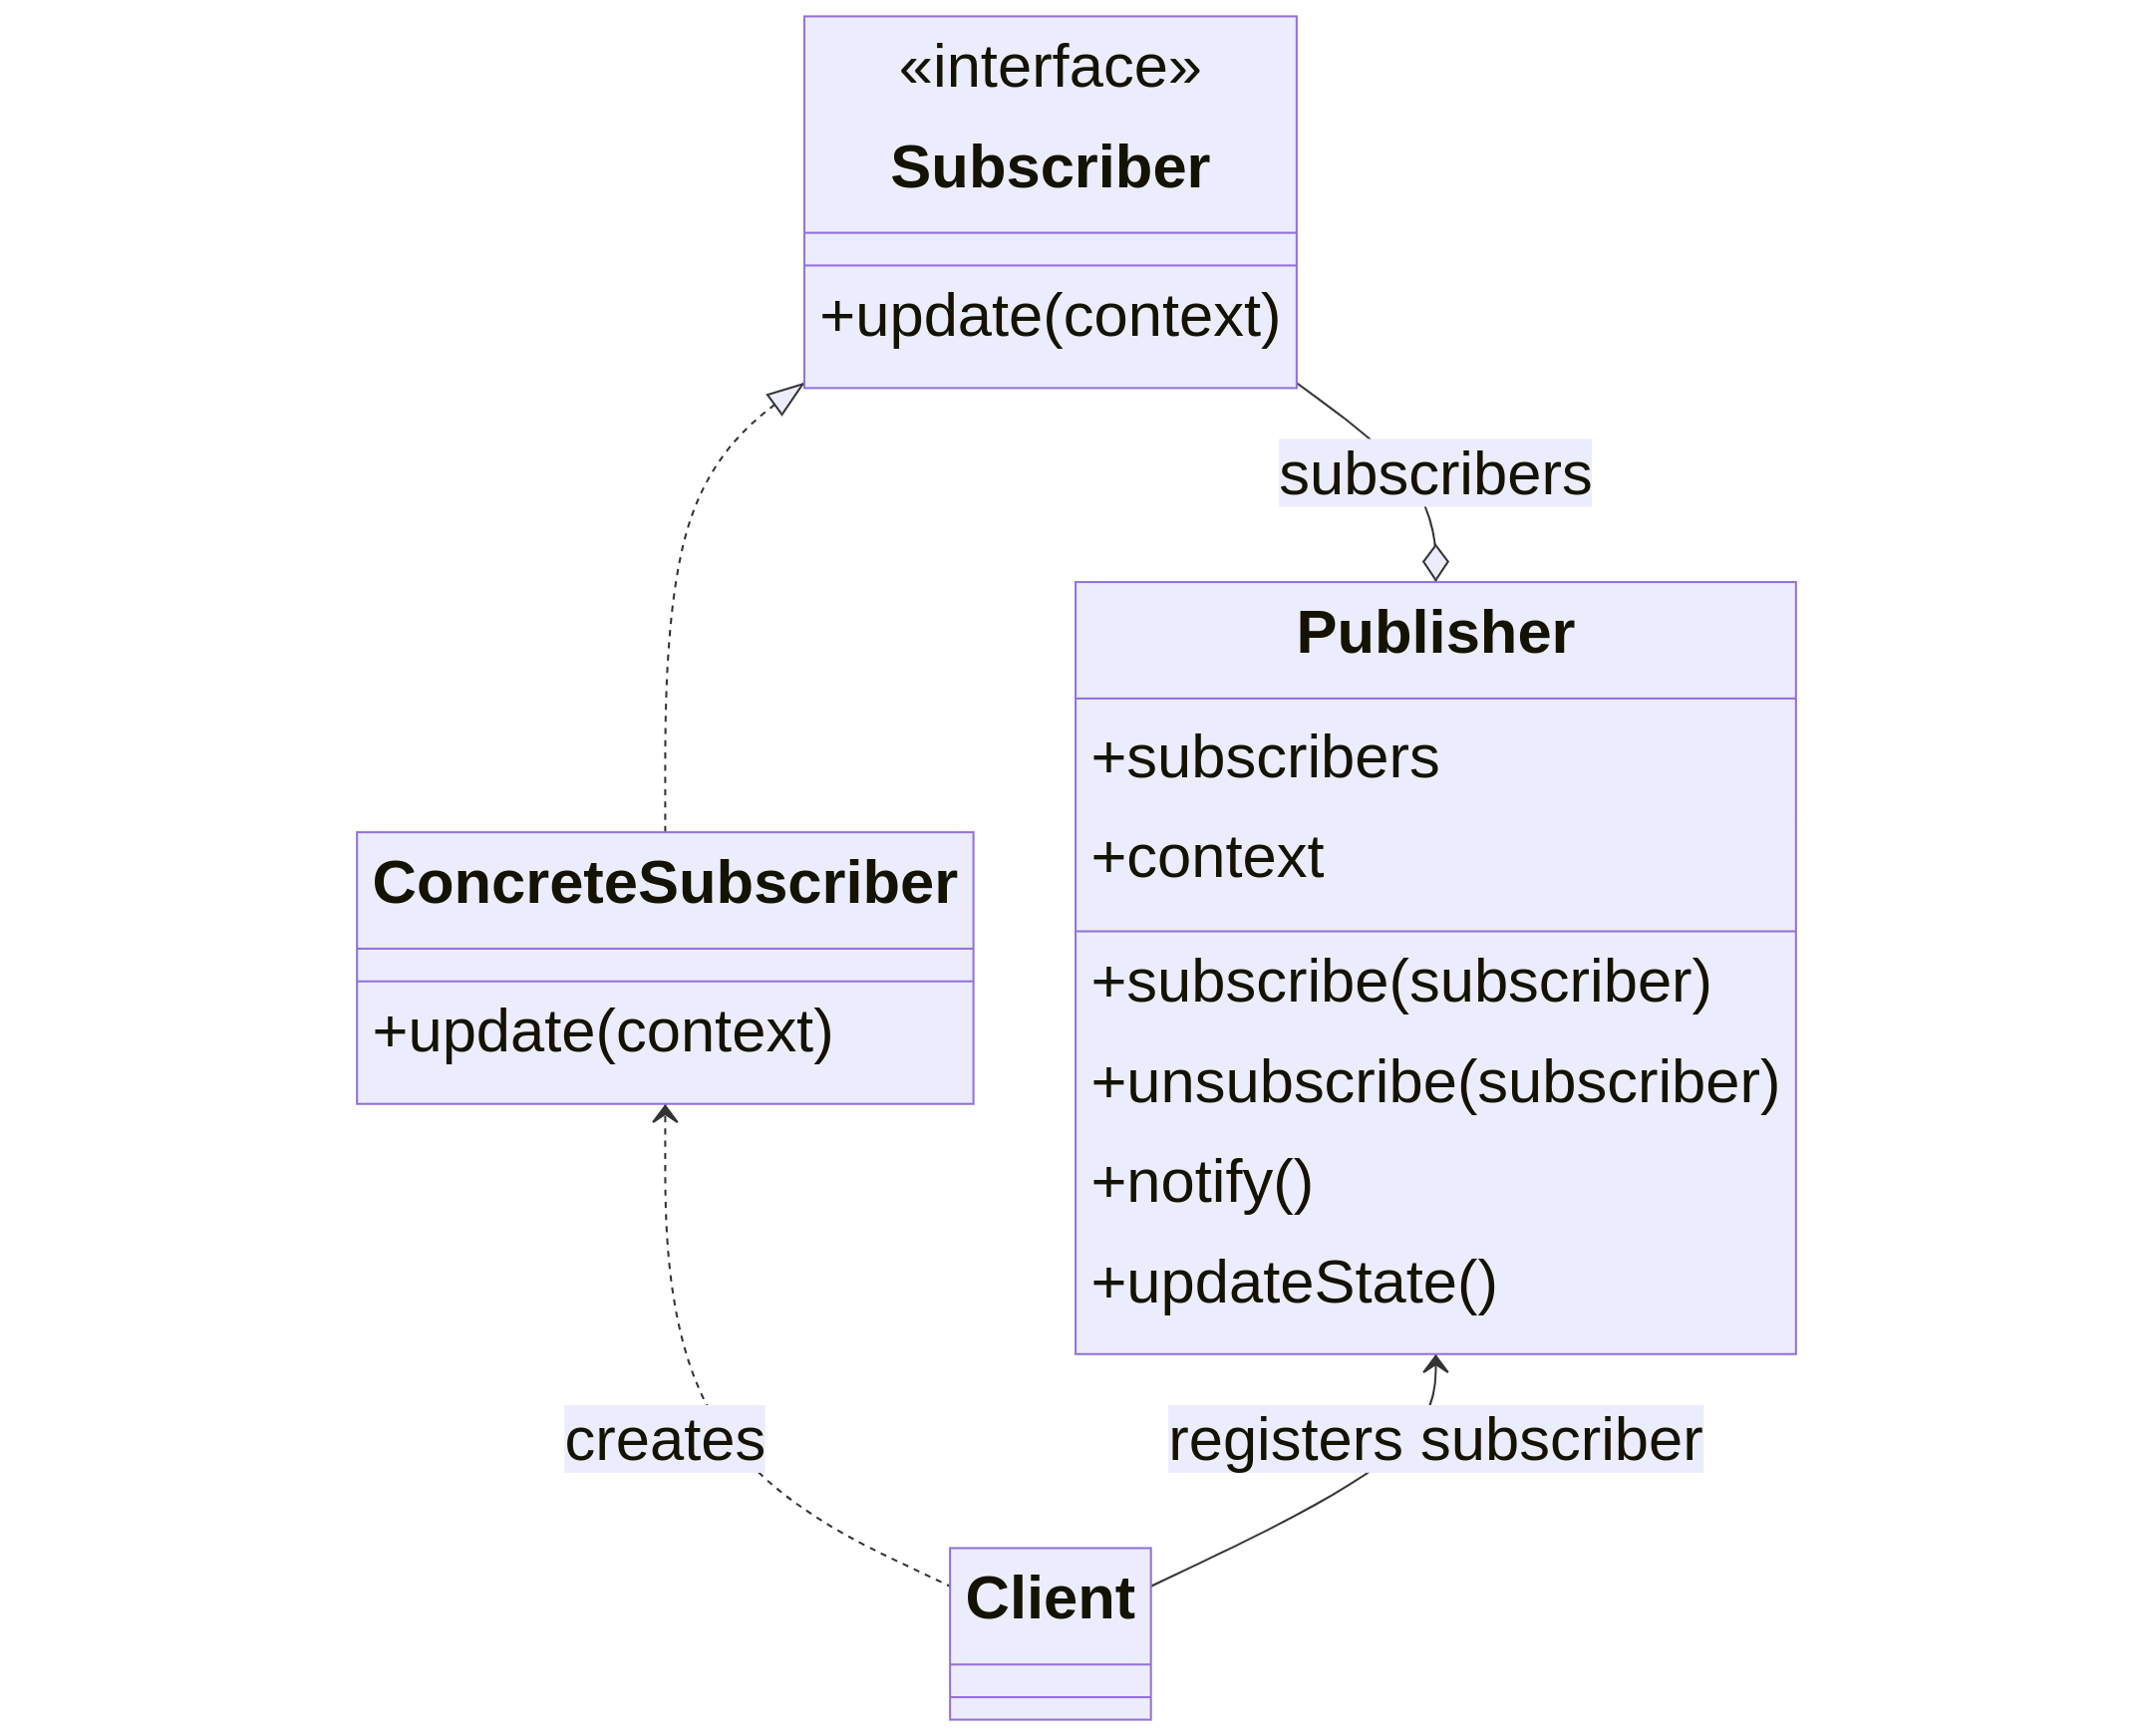
\includegraphics[width=0.75\linewidth]{images/patterns/observer-class.png}
	\caption{Klassendiagramm Observer}
	\label{fig:observer-class}
\end{figure}

Der Client kann den Zustand des Publishers durch Senden von `updateSate` verändern (1). Der Publisher sendet sich draufhin selbst `notify` (2) und beginnt über seine Liste von Subscribern zu iterieren. Jedem Subscriber sendet er dann `update` (3, 5) und übergibt den notwendigen Kontext, sodass der Subscriber seinen Zustand entsprechend aktualisieren kann. 

\begin{figure}[!hb]
	\centering
	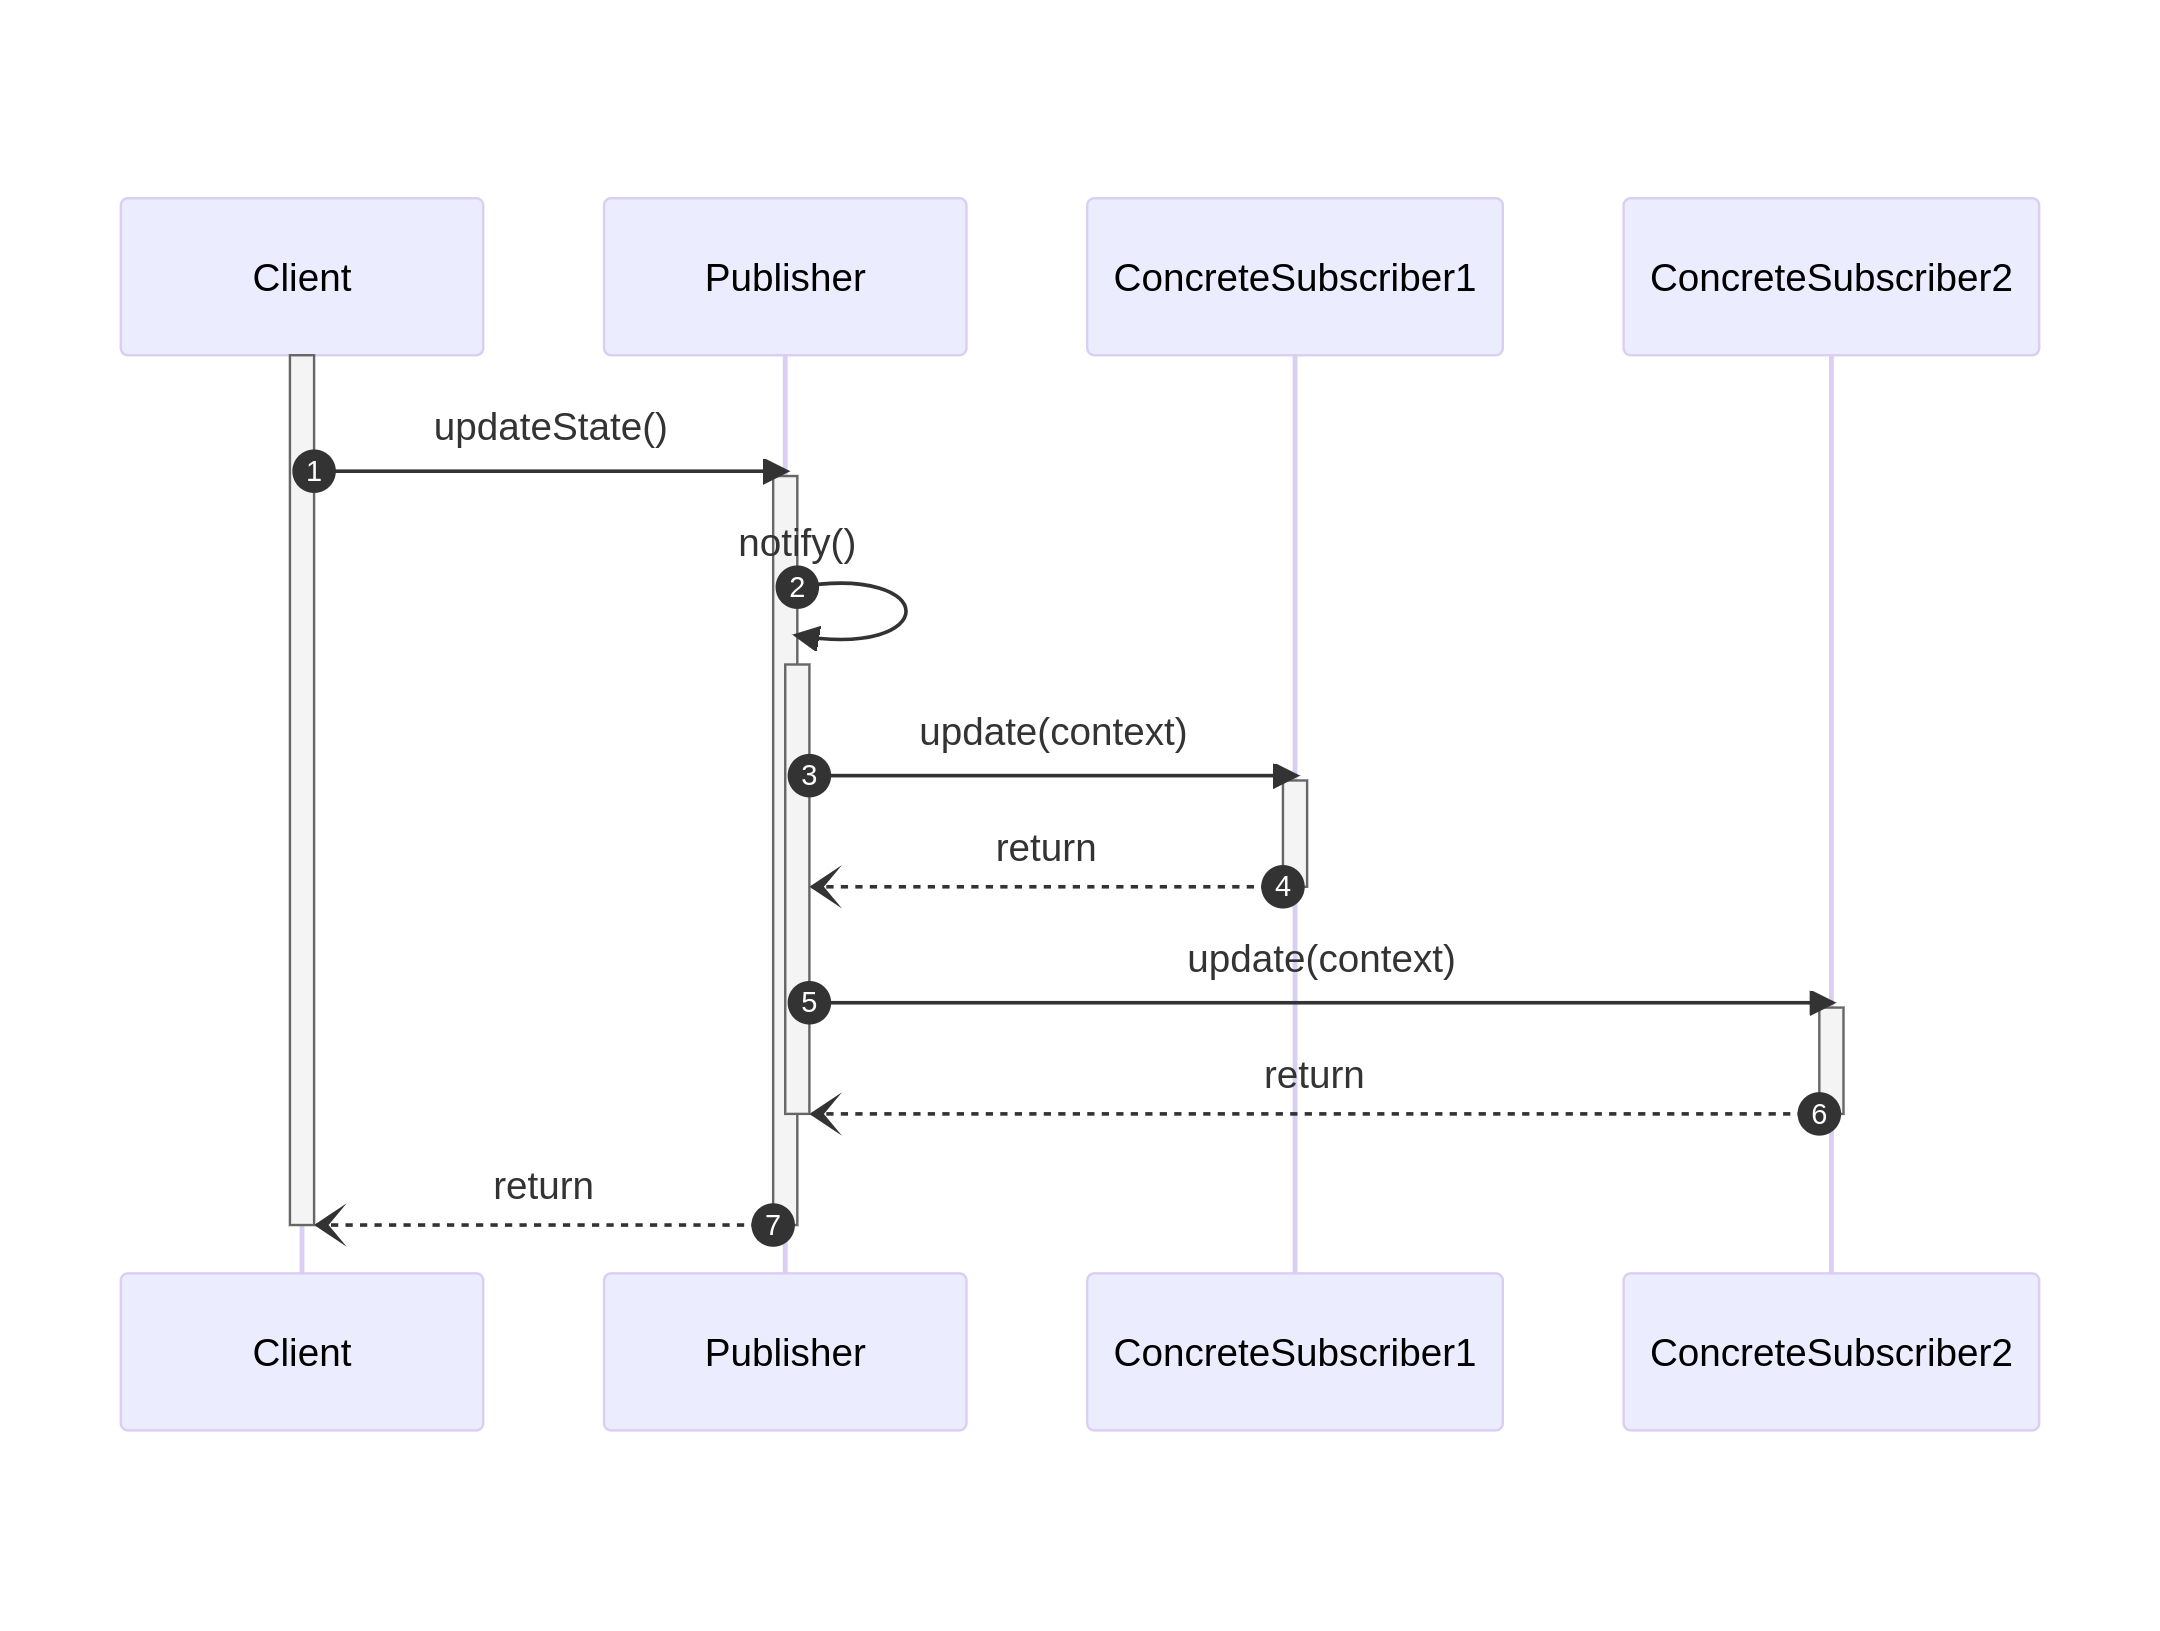
\includegraphics[width=0.75\linewidth]{images/patterns/observer-seq.png}
	\caption{Sequenzdiagramm Observer}
	\label{fig:observer-seq}
\end{figure}

Der folgende Code veranschaulicht die Benachrichtigung aller Subscriber. In `notify` wird an jeden im Publisher referenzierten Subscriber `update` gesendet. Dabei wird der Kontext des Publishers an jeden Subscriber übergeben.

\lstset{language=python}
\begin{lstlisting}[caption={Quelltextunterschrift}, label=code:template-method-code]
class Publisher
	def notify(self):
        for subscriber in self.subscribers:
            subscriber.update(self.context)
\end{lstlisting}


\subsubsection*{Konsequenzen}

Template Methods sind ein Mechanismus, welcher die Wiederverwendung von Code ermöglicht und kann somit der Codeduplikation entgegen wirken. Anstatt Das Observer-Pattern bietet eine Reihe von Vorteilen. Durch Separation von Publisher und Subscriber und durch die Abstraktion des Subscriber-Interfaces wird eine lose Kopplung der beiden erreicht. Diese lose Kopplung ermöglicht es, sowohl den Publisher, als auch die Subscriber beliebig auszutauschen. Weiterhin können sich der Publisher und die Subscriber auf unterschiedlichen Abstraktionsniveaus befinden. Ein Publisher auf einem niedrigen Level kann einen Subscriber auf einem hohen Level benachrichtigen. Wären Subscriber und Publisher nicht getrennt, so wäre dafür ein Abstraktionshierarchie-übergreifendes Objekt notwendig, welches die Trennung der Abstraktionsschichten beeinträchtigen würde. Ein weiterer Vorteil ist die dynamische Anzahl der Subscriber, mit denen ein Publisher interagieren kann. So kann der Client über den Publisher eine beliebige Zahl an Subscribern erreichen.

Ein Nachteil des Observer-Patterns ist, dass der Publisher stets alle seine Subscriber benachrichtigt. Es kann vorkommen, dass nur eine Teilmenge der Subscriber die Benachrichtigung benötigt, was in unnötigen Methodenaufrufen resultiert.